%%%%%%%% mlsys 2024 EXAMPLE LATEX SUBMISSION FILE %%%%%%%%%%%%%%%%%

\documentclass{article}

% Recommended, but optional, packages for figures and better typesetting:
\usepackage{microtype}
\usepackage{graphicx}
\usepackage{subfigure}
\usepackage{booktabs} % for professional tables

% hyperref makes hyperlinks in the resulting PDF.
% If your build breaks (sometimes temporarily if a hyperlink spans a page)
% please comment out the following usepackage line and replace
% \usepackage{mlsys2024} with \usepackage[nohyperref]{mlsys2024} above.
\usepackage{hyperref}

% Attempt to make hyperref and algorithmic work together better:
\newcommand{\theHalgorithm}{\arabic{algorithm}}

% Use the following line for the initial blind version submitted for review:
\usepackage{mlsys2024}

% For code listings
\usepackage{sourcecodepro}
\usepackage[T1]{fontenc}
\usepackage{listings}
\usepackage[dvipsnames]{xcolor}
\definecolor{commentgreen}{RGB}{2,112,10}
\definecolor{eminence}{RGB}{108,48,130}
\definecolor{weborange}{RGB}{255,165,0}
\definecolor{frenchplum}{RGB}{129,20,83}
%Define Colors
\definecolor{gray}{RGB}{102,102,102}		%#666666
\definecolor{lightblue}{RGB}{0,102,153}		%#006699
\definecolor{lightgreen}{RGB}{102,153,0}	%#669900
\definecolor{bluegreen}{RGB}{51,153,126}	%#33997e
\definecolor{magenta}{RGB}{217,74,122}		%#d94a7a
\definecolor{orange}{RGB}{226,102,26}		%#e2661a
\definecolor{purple}{RGB}{125,71,147}		%#7d4793
\definecolor{green}{RGB}{113,138,98}		%#718a62

\usepackage{tikz}
\usetikzlibrary{positioning, fit, backgrounds}

\usepackage[framemethod=tikz]{mdframed}
\lstdefinelanguage{Wave}{
    language=Python,
    classoffset=1,
    morekeywords={WorkgroupConstraint, TilingConstraint, WaveConstraint, HardwareConstraint},
    keywordstyle=\color{lightblue},
    classoffset=2,
    morekeywords={Memory, Register},
    keywordstyle=\color{lightgreen},
    classoffset=3,
    morekeywords={reduction, read, write, mma},
    keywordstyle=\color{magenta},
    classoffset=4,
    morekeywords={@wave, @reduction},
    keywordstyle=\color{orange},
    sensitive=false, % keywords are not case-sensitive
}

\lstset{
  language={Wave},
  basicstyle={\scriptsize\ttfamily},
  identifierstyle={\scriptsize\ttfamily},
  commentstyle={\scriptsize\itshape\ttfamily},
  keywordstyle={\scriptsize\bfseries\ttfamily},
  ndkeywordstyle={\scriptsize\ttfamily},
  stringstyle={\scriptsize\ttfamily},
  frame={tb},
  breaklines=true,
  columns=[l]{fullflexible},
  xrightmargin=0em,
  xleftmargin=0em,
  numberstyle={\scriptsize},
  stepnumber=1,
  numbersep=1em,
  lineskip=-0.5ex,
}

% If accepted, instead use the following line for the camera-ready submission:
% \usepackage[accepted]{mlsys2024}

% The \mlsystitle you define below is probably too long as a header.
% Therefore, a short form for the running title is supplied here:
\mlsystitlerunning{Submission and Formatting Instructions for MLSys 2024}

\begin{document}

\twocolumn[
\mlsystitle{Wave : A Symbolic Python DSL and Compiler for High Performance Machine Learning}

% It is OKAY to include author information, even for blind
% submissions: the style file will automatically remove it for you
% unless you've provided the [accepted] option to the mlsys2024
% package.

% List of affiliations: The first argument should be a (short)
% identifier you will use later to specify author affiliations
% Academic affiliations should list Department, University, City, Region, Country
% Industry affiliations should list Company, City, Region, Country

% You can specify symbols, otherwise they are numbered in order.
% Ideally, you should not use this facility. Affiliations will be numbered
% in order of appearance and this is the preferred way.
\mlsyssetsymbol{equal}{*}

\begin{mlsysauthorlist}
\mlsysauthor{Aeiau Zzzz}{equal,to}
\mlsysauthor{Bauiu C.~Yyyy}{equal,to,goo}
\mlsysauthor{Cieua Vvvvv}{goo}
\mlsysauthor{Iaesut Saoeu}{ed}
\mlsysauthor{Fiuea Rrrr}{to}
\mlsysauthor{Tateu H.~Yasehe}{ed,to,goo}
\mlsysauthor{Aaoeu Iasoh}{goo}
\mlsysauthor{Buiui Eueu}{ed}
\mlsysauthor{Aeuia Zzzz}{ed}
\mlsysauthor{Bieea C.~Yyyy}{to,goo}
\mlsysauthor{Teoau Xxxx}{ed}
\mlsysauthor{Eee Pppp}{ed}
\end{mlsysauthorlist}

\mlsysaffiliation{to}{Department of Computation, University of Torontoland, Torontoland, Canada}
\mlsysaffiliation{goo}{Googol ShallowMind, New London, Michigan, USA}
\mlsysaffiliation{ed}{School of Computation, University of Edenborrow, Edenborrow, United Kingdom}

\mlsyscorrespondingauthor{Cieua Vvvvv}{c.vvvvv@googol.com}
\mlsyscorrespondingauthor{Eee Pppp}{ep@eden.co.uk}

% You may provide any keywords that you
% find helpful for describing your paper; these are used to populate
% the "keywords" metadata in the PDF but will not be shown in the document
\mlsyskeywords{Machine Learning, MLSys}

\vskip 0.3in

\begin{abstract}
This document provides a basic paper template and submission guidelines.
Abstracts must be a single paragraph, ideally between 4--6 sentences long.
Gross violations will trigger corrections at the camera-ready phase.
\end{abstract}
]

% this must go after the closing bracket ] following \twocolumn[ ...

% This command actually creates the footnote in the first column
% listing the affiliations and the copyright notice.
% The command takes one argument, which is text to display at the start of the footnote.
% The \mlsysEqualContribution command is standard text for equal contribution.
% Remove it (just {}) if you do not need this facility.

%\printAffiliationsAndNotice{}  % leave blank if no need to mention equal contribution
\printAffiliationsAndNotice{\mlsysEqualContribution} % otherwise use the standard text.

\section{Introduction}
Generative models have seen tremendous success in a wide variety of
domains ranging from image generation to natural language processing and beyond.
\cite{podell_sdxl_2023,dubey_llama_2024}. Much of this success is being
driven by graphics processing units (GPUs) which while originally
designed for graphics, are now being optimized for machine learning.
Both datacenter and consumer grade GPUs feature powerful matrix multiplication hardware units
and specialized instructions to enable high performance inference and training \cite{sun_dissecting_2023}.
\\ \\
Given the importance of GPUs in machine learning, significant
effort has been put into developing frameworks that allow developers to
write high performance machine learning models with a low barrier to entry. Frameworks such
as Pytorch \cite{paszke_pytorch_2019} have become extremely popular
because they expose a Python based approach to programming GPUs. Prior
to the advent of these frameworks, developers had to write CUDA or OpenCL
kernels by hand which required significant expertise to achieve
good performance and did not scale well to new operators.
\\ \\
Under the hood, these machine learning frameworks rely heavily
on vendor-specific libraries such as cuDNN \cite{chetlur_cudnn_2014} to achieve high performance.
These libraries are performant but are black boxes consisting of
hand-written kernels and often do not support the full set of
operators encountered in machine learning models.
To address these limitations, recent work has focused on developing
Python domain specific languages (DSL) that allow developers to get high performance
while reducing the kernel complexity. Triton \cite{tillet_triton_2019}.
is a popular Python DSL that exposes a workgroup level programming
model and allows developers to author high performance kernels.
In the programmability versus performance tradeoff, Triton demonstrated that it is possible to
achieve high performance while maintaining a high level of programmability. However,
Triton kernels often get quite complex as the kernel complexity grows. Most of this complexity
comes from exposing a pointer based approach to access and manipulate memory.
\\ \\
In this paper, we introduce Wave, a Python DSL and compiler for high performance machine learning.
Wave exposes a subgroup (wave or warp) level programming model and uses constraints
to specify the distribution strategy for the kernel. This allows for a separation between
the kernel and distribution strategy and results in simpler kernels. The language
and compiler make extensive use of symbolic data types to represent tensor shapes and memory access patterns
that make it easier to reason about the kernel. We demonstrate that Wave can achieve competitive performance
with Triton and hand-tuned kernels on core machine learning operators such as matrix multiplication,
convolutions and attention.
In summary, the contributions of this paper are as follows:
\begin{itemize}
    \item \textbf{Wave language} (Section \ref{section:wave_language}): A Python DSL that exposes a subgroup programming model for GPUs. The language
    defines constraints that separate distribution strategies from the description of the core computation. Tensor shapes and address spaces
    are represented using symbolic types (using sympy).
    \item \textbf{Wave compiler} (Section \ref{section:wave_compiler}): A Python compiler that uses symbolic types
    to represent memory access patterns and reason about them. The compiler uses torch.fx to trace the kernel,
    then runs a series of compiler optimization passes and finally lowers the computation graph to MLIR and LLVM.
    \item \textbf{Numerical Experiments} (Section \ref{section:numerical_experiments}): Numerical experiments on
    matrix multiplication, convolutions and attention that demonstrate the performance of Wave kernels and show
    that it is on par with existing DSLs and hand-tuned libraries.

\end{itemize}

\section{Wave Language}
In this section, we will go through the Wave language and its features using matrix multiplication as an example. See Listing \ref{lst:gemm} for the full code listing.

\label{section:wave_language}
\subsection{Wave Programming Model}
Wave programs follow the single-program multiple data (SPMD) programming model where the kernel is written
at the level of execution of a single wave or warp. While waves are core to how programs are executed on
GPUs, most GPU languages do not expose them directly to the developer. CUDA, for example, allows workgroup
and thread level programming but does not expose the wave level while Triton only exposes workgroup level programming.
The advantages of the wave programming model are that it allows developers to write kernels at the same level of
abstraction as the native hardware matrix multiply accumulate (MMA) instructions which operate at the granularity of waves
giving them low-level control from a high-level abstraction.
% Should we compare to the Triton programming model here?
% Possibly we could have roughly something like figure 3 of the Triton paper

\subsection{Syntax \& Semantics}
The Wave language partitions programs into two distinct regions as can be seen in Listing \ref{lst:gemm}.
The first part of the program consists of constraints which are new constructs introduced by the language.

\subsubsection{Constraints}
Constraints are used to represent the distribution strategy of a kernel. Each constraint operates on a particular
dimension and specifies how that dimension is to be distributed. In the matrix multiplication example of Listing \ref{lst:gemm},
the \texttt{WorkgroupConstraint} on symbolic dimension \texttt{M/N} states that the \texttt{M/N} dimension is distributed among work group dimension 0/1
with a tile size of \texttt{BLOCK\_M/BLOCK\_N}. The \texttt{WaveConstraint} on the \texttt{M/N} dimension states that the $M/N$ dimension is then further distributed among waves
with a tile size of \texttt{BLOCK\_M / 2 / BLOCK\_N / 2}. The \texttt{TilingConstraint} on \texttt{K} specifies that the \texttt{K} dimension is tiled with a tile size of \texttt{BLOCK\_K}
in a sequential for loop. Finally, the \texttt{HardwareConstraint} specifies hardware specific parameters such as the number of threads per wave, the number of waves per block and
the canonical shape of the program.
\\ \\
The canonical shape of the program specifies the minimum granularity of the operations in the program. In the matrix multiplication example and for programs using MMA instructions, the canonical shape is
the shape of the MMA instruction which is \texttt{M = 16, N = 16, K = 16}. For programs that do not use MMA instructions, users can
explicitly specify the canonical shape of the program in the \texttt{HardwareConstraint} by using the \texttt{vector\_shapes} keyword. For more examples of this,
see Appendix \ref{appendix:samples}.
\\ \\
The constraints of the program serve multiple purposes. First, they separate out the distribution strategy from the kernel.
Second, they result in much simpler kernels because kernel authors do not need to keep track the offsets to different memory locations
as the compiler takes care of this.

\subsubsection{Kernel}
The kernel is the second part of the program and consists of the core computation. It is annotated with the \texttt{@wave} decorator which
is used by the compiler to trace the kernel. In the matrix multiplication example, the inputs to the kernel are of type \texttt{Memory} which
represents a memory buffer with a symbolic shape and address space (shared memory or global memory). In the kernel,
even though the inputs are specified as type \texttt{Memory} with shape \texttt{[M, K], [N, K], [M, N]}, the actual shape of the memory
is determined by the constraints. In order to simplify the kernel, we write the kernel using the original symbolic shapes and let the compiler
determine the actual shapes of the memory buffers.
% Note: The question that comes up with this phrasing: Could these shapes then just be left out. In reality they are at least important to figure out the indexing dimensions.

\begin{lstlisting}[language=Wave, frame=single, breaklines, caption={Mixed-precision $C = A \times B^{T}$ expressed in Wave.}, captionpos=b, label={lst:gemm}]
constraints = [WorkgroupConstraint(M, BLOCK_M, 0)]
constraints += [WorkgroupConstraint(N, BLOCK_N, 1)]
constraints += [TilingConstraint(K, BLOCK_K)]
constraints += [WaveConstraint(M, BLOCK_M / 2)]
constraints += [WaveConstraint(N, BLOCK_N / 2)]
constraints += [
    HardwareConstraint(threads_per_wave=64,
    waves_per_block=(2, 2, 1),
    mma_type=MMAType.F32_16x16x16_F16
]

@wave(constraints)
def gemm(
    a: Memory[M, K, ADDRESS_SPACE, f16],
    b: Memory[N, K, ADDRESS_SPACE, f16],
    c: Memory[M, N, GLOBAL_ADDRESS_SPACE, f32],
):
    c_reg = Register[M, N, f32](0.0)

  @reduction(K, init_args=[c_reg])
  def loop(acc: Register[M, N, f32]) -> Register[M, N, f32]:
      a_reg = read(a, elements_per_thread=ELEMS)
      b_reg = read(b, elements_per_thread=ELEMS)
      acc = mma(a_reg, b_reg, acc)
      return acc

  write(loop, c, elements_per_thread=ELEMS)
\end{lstlisting}

The next type in wave is the \texttt{Register} type which represents a virtual
register. Most of the operations in the kernel operate on \texttt{Register} types.
In this particular example, we instantiate a register \texttt{c\_reg} of shape \texttt{[M, N]}
and type \texttt{f32} and initialize it to 0.0. The \texttt{Register} type is used as the accumulator in the \texttt{K} loop
of matrix multiplication.

We then define a \texttt{reduction} operator which defines a reduction loop over the
\texttt{K} dimension. The \texttt{reduction} operator takes any number of \texttt{Register} types as accumulators and
can be thought of as the equivalent of a \texttt{for} loop. The step size and bounds of the loop are determined by the
constraints. Within the \texttt{reduction} operator, we read from the input memory buffers \texttt{a} and \texttt{b} using
the \texttt{read} operator and perform a matrix multiply accumulate operation using the \texttt{mma} operator. The \texttt{mma}
operator maps to the MMA instruction specified in the \texttt{HardwareConstraint}. Variables defined outside the \texttt{reduction}
are accessible within the \texttt{reduction}. The result of the \texttt{reduction} can be accessed by the name of the function \texttt{loop}.

Finally, we write the result of the reduction loop to the output memory buffer \texttt{c} using the \texttt{write} operator. Both the \texttt{read} and \texttt{write} operators
support several additional arguments such as \texttt{elements\_per\_thread} and \texttt{mapping}. The \texttt{elements\_per\_thread} argument specifies the number of elements
that each thread should load and can be thought of as a compiler hint that makes it easier for the compiler to go from the wave description of the program
to the thread description of the program.
\\ \\
TODO(Ivan): Add description of mapping argument here with examples.

\newpage

\section{Wave Compiler}
\label{section:wave_compiler}
The Wave compiler is a Python-based compiler designed to process and optimize kernels written in the Wave language. It leverages symbolic types to represent memory access patterns and perform reasoning about them. The compilation process involves several key steps:

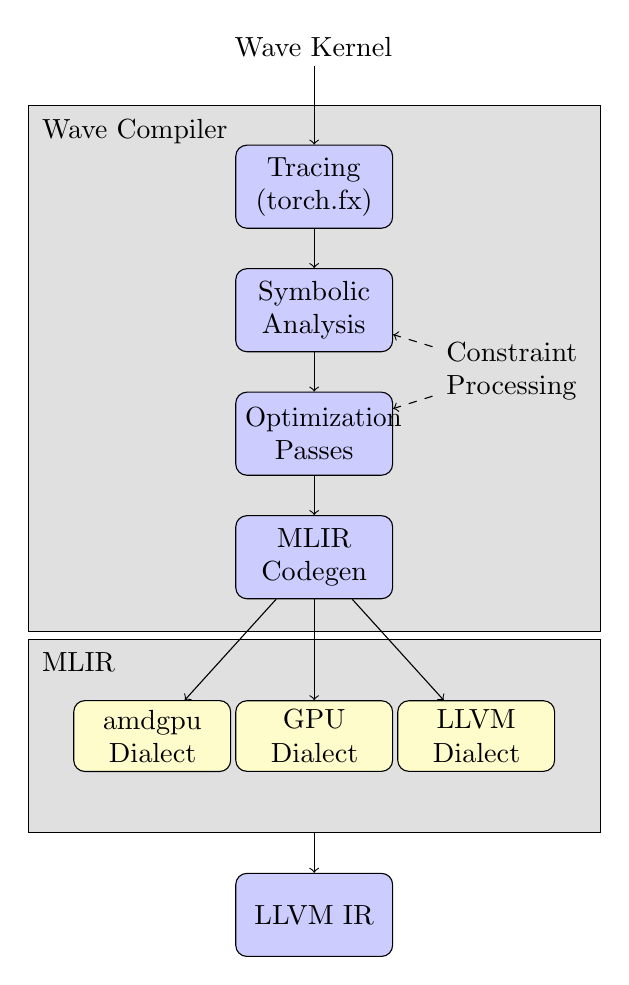
\begin{tikzpicture}[node distance=0.5cm, auto]
    % Define styles
    \tikzstyle{block} = [rectangle, draw, fill=blue!20,
        text width=5em, text centered, rounded corners, minimum height=3em]
    \tikzstyle{mlir} = [rectangle, draw, fill=gray!20,
        text width=20em, text centered, minimum height=7em]
    \tikzstyle{wave_compiler} = [rectangle, draw, fill=gray!20,
        text width=20em, text centered, minimum height=19em]
    \tikzstyle{dialect} = [rectangle, draw, fill=yellow!20,
        text width=5em, text centered, rounded corners, minimum height=2em]
    \tikzstyle{line} = [draw, ->]

    % Place nodes

    \node [text width=10em, text centered] (wave) {Wave Kernel};

    \node [wave_compiler, below=of wave] (wave_compiler) {};
    \node [anchor=north west, inner sep=0.5em] at (wave_compiler.north west) {Wave Compiler};

    \node [block, below=1cm of wave] (tracing) {Tracing (torch.fx)};
    \node [block, below=of tracing] (symbolic) {Symbolic Analysis};
    \node [block, below=of symbolic] (optimization) {Optimization Passes};
    \node [block, below=of optimization] (mlir_codegen) {MLIR Codegen};

    % MLIR box with dialects
    \node [mlir, below=of mlir_codegen] (mlir) {};
    \node [anchor=north west, inner sep=0.5em] at (mlir.north west) {MLIR};
    \node [dialect, left=3em of mlir.center] (dialect1) {amdgpu Dialect};
    \node [dialect, at=(mlir.center)] (gpu_dialect) {GPU Dialect};
    \node [dialect, right=3em of mlir.center] (llvm_dialect) {LLVM Dialect};
    \node [block, below=of mlir] (llvm) {LLVM IR};

    % Draw edges
    \path [line] (wave) -- (tracing);
    \path [line] (tracing) -- (symbolic);
    \path [line] (symbolic) -- (optimization);
    \path [line] (optimization) -- (mlir_codegen);
    \path [line] (mlir_codegen) -- (dialect1);
    \path [line] (mlir_codegen) -- (gpu_dialect);
    \path [line] (mlir_codegen) -- (llvm_dialect);

    \path [line] (mlir) -- (llvm);

    % Add a note about constraints
    \node [text width=5em, text centered, below right=-0.25cm and 0.5cm of symbolic] (constraints) {Constraint Processing};
    \draw [dashed, ->] (constraints) -- (symbolic);
    \draw [dashed, ->] (constraints) -- (optimization);
\end{tikzpicture}

\subsection{Tracing with torch.fx}

The Wave compiler utilizes torch.fx~\cite{reed2022torch} for symbolic tracing of the kernel. This process involves executing the Python kernel program with special \emph{Proxy} objects that act as placeholders for actual values. As the program runs, torch.fx records all definitions and function calls, effectively capturing the computational structure of the kernel. The result is a comprehensive representation of the kernel's logic in the form of the torch.fx graph IR. By leveraging torch.fx, Wave strikes a balance between the flexibility of a Python-embedded DSL and the power of a custom compiler, allowing for specialized optimizations while maintaining an accessible and extensible programming model.

\subsection{Intermediate Representation}
We extended the torch.fx intermediate representation with custom primitives and types to accurately model the Wave programming model. Our enhancements include custom primitives representing Wave-specific constructs such as wave-level operations and memory accesses. Representing them explicitly in the IR simplifies type inference and enables easier transformations on the IR. At the same time we keep compatibility with torch.fx IR in order to reuse existing tooling for e.g. visualization.


\subsection{Lowering Wave programming to thread programming}
% Note: A description of the programming model will already be in the previous chapter. So I can take that as a given.
A wave kernel is expressed following an SPMD programming model in the granularity of a single wave. While the target programming model for the output IR follows SPMD as well, it operates on the granularity of a single thread with explicit data movement and synchronization.
In consequence the computation graph needs to be expanded according to the input sizes and the distribution of data to threads to model the instructions for each thread.
\smallskip
As each thread has to load different data depending on its position in the launch grid %or do we call this differently?
we prepend the IR with operations to get the \texttt{\footnotesize thread\_id} and \texttt{\footnotesize workgroup\_id} for the relevant dimensions.

First, we determine to which level each dimension has to expand according to the input sizes and constraints.
% small example?
We start at the leaf nodes of the kernel and follow def-uses upward until we reach the kernel inputs. We each node we reach we:
\begin{enumerate}
    \item Determine the dimensions this node needs to index in
    \item \ldots
\end{enumerate}
% TODO: Preliminary, maybe better to just express this as an algorihm?

% TODO: Can we produce a figure (or graph) of pre-expansion and post-expansion? Maybe only expansion in a single dimension if this gets too large otherwise?


% Thought:
% We name this programming model \emph{SIWT} (Single Instruction, Wave of Threads) denoting that a single instruction is executed by a wave of threads. This is inspired by the SIMT execution model where instructions are executed by all threads in lockstep.


\subsection{Instruction Scheduling}
% Describe the deep type of decisions we can take already on this level with the vast information we still have available
One of the advantages of simpler kernels is that the compiler can make some high-level scheduling decisions at this level before
handing it off to and pre and post-register allocation scheduling passes in the LLVM backend. For example, in the matrix multiplication example,
since the kernel only consists of reads, writes and matrix multiply accumulate operations, the compiler can pipeline these instructions based on
a tunable cost metric. We use vanilla modulo scheduling \cite{dragonbook} to schedule the kernels. We expose the number of shared memory,
global memory and MMA units as well as delays associated with their corresponding instructions as tunable parameters to the compiler.
In order to enforce our schedule, we use LLVM scheduling barrier intrinsics \texttt{llvm.amdgcn.sched\_group.barrier} that uses linear programming
to enforce the schedule. The tunable parameters allow us to balance the register pressure with the instruction level parallelism.


\subsection{Optimization Passes}
After tracing, the compiler executes a series of optimization passes on the computational graph, such as:
\textbf{barrier insertion} % We could give more specifics here on when we insert barriers
\ldots

\subsection{Lowering to MLIR}

% TODO: mention symbolic types, their optimization and lowering here
% Also mention for which sizes we use them: Tensor shapes, ...
% basically the sympy walker we have.

The final stage of the compilation process involves lowering the optimized computational graph to several MLIR dialects: % TODO: possibly present this differently, for now a list is fine.
%We target the amdgpu and gpu dialects to model GPU

% Possibly simplify if this is too specific
\begin{itemize}
    \item Intrinsics used in the kernel are directly mapped to operations of the \texttt{\footnotesize amdgpu} dialect
    \item The \texttt{\footnotesize gpu} dialect is used to model general GPU concepts, such as \texttt{\footnotesize thread\_id}
    \item The \texttt{\footnotesize scf} dialect is used to model loops
    \item The \texttt{\footnotesize llvm} dialect is used to emit scheduling barriers that preserve our instruction scheduling decisions
    \item We use the \texttt{\footnotesize scf}, \texttt{\footnotesize arith}, and \texttt{\footnotesize math} dialects to model loops and arithmetic.
    \item Furthermore we use the \texttt{\footnotesize memref} and \texttt{\footnotesize func} dialects
\end{itemize}



% mention LLVM scheduling barriers

\subsection{Integration}
TODO: briefly describe integration into Pytorch (compile to vmfb + call with torch tensors) \& IREE (\ldots)?



\bigskip
In summary, the Wave compiler combines symbolic computation, multi-stage lowering, and GPU-specific optimizations to translate high-level Wave kernels into efficient, low-level code suitable for execution on GPUs. Its use of symbolic types and constraint-based programming model allows for powerful optimizations while maintaining a high level of abstraction for kernel developers.

\section{Numerical Experiments}
\label{section:numerical_experiments}
In this section, we present results from our experiments on the MI300. Specifically, we evaluate the performance of Wave on three core ML operators: matrix multiplication, convolutions, and attention.
We compare against Triton and other libraries such as PyTorch and IREE.

\subsection{Matrix Multiplication}
We compute matrix multiplication $C = A \times B^{T}$ using mixed-precision
arithmetic. The inputs are in \texttt{fp16} while the output is in \texttt{fp32}.
We pick the matrix shapes from the SDXL model \cite{podell2023sdxlimprovinglatentdiffusion}.
We compare the performance of the Wave kernel against Triton and PyTorch. The results are shown in Figure \ref{fig:gemm_results}.
\\ \\
From the results, we see that Wave outperforms Triton on all shapes and is faster
than PyTorch for all except two shapes.


\begin{figure}[htbp]
    \def\svgwidth{0.5\textwidth}
    \input{gemm_performance.pdf_tex}
    \caption{GEMM Performance Results}
    \label{fig:gemm_results}
\end{figure}

\subsection{Convolution}
\subsection{Attention}

\section{Related Work}
\label{section:related_work}

\section{Conclusions \& Future Work}
\label{section:conclusions}

\section{Acknowledgements}
\label{section:acknowledgements}

\section{Appendix: Sample Wave Programs}
\label{section:samples}

\section{Appendix: Experiment Details}
TODO - Decide whether we want to keep this section.
\label{section:details}
\subsection{Matrix Multiplication}
\subsubsection{Triton \& PyTorch Benchmarking}
We use 53166efa2494764e11734d57de681cc4d2486981 commit of Triton for our experiments and Pytorch 2.3.0a0+git1b935e2. We use the following command to run the matrix multiplication benchmark:
\begin{lstlisting}
  python 03-matrix-multiplication.py
\end{lstlisting}
The triton file for the test is attached below.
\begin{lstlisting}
    """
    Matrix Multiplication
    =====================
    In this tutorial, you will write a very short high-performance FP16 matrix multiplication kernel that achieves
    performance on par with cuBLAS or rocBLAS.

    You will specifically learn about:

    * Block-level matrix multiplications.

    * Multi-dimensional pointer arithmetic.

    * Program re-ordering for improved L2 cache hit rate.

    * Automatic performance tuning.

    """

    # %%
    # Motivations
    # -----------
    #
    # Matrix multiplications are a key building block of most modern high-performance computing systems.
    # They are notoriously hard to optimize, hence their implementation is generally done by
    # hardware vendors themselves as part of so-called "kernel libraries" (e.g., cuBLAS).
    # Unfortunately, these libraries are often proprietary and cannot be easily customized
    # to accommodate the needs of modern deep learning workloads (e.g., fused activation functions).
    # In this tutorial, you will learn how to implement efficient matrix multiplications by
    # yourself with Triton, in a way that is easy to customize and extend.
    #
    # Roughly speaking, the kernel that we will write will implement the following blocked
    # algorithm to multiply a (M, K) by a (K, N) matrix:
    #
    #  .. code-block:: python
    #
    #    # Do in parallel
    #    for m in range(0, M, BLOCK_SIZE_M):
    #      # Do in parallel
    #      for n in range(0, N, BLOCK_SIZE_N):
    #        acc = zeros((BLOCK_SIZE_M, BLOCK_SIZE_N), dtype=float32)
    #        for k in range(0, K, BLOCK_SIZE_K):
    #          a = A[m : m+BLOCK_SIZE_M, k : k+BLOCK_SIZE_K]
    #          b = B[k : k+BLOCK_SIZE_K, n : n+BLOCK_SIZE_N]
    #          acc += dot(a, b)
    #        C[m : m+BLOCK_SIZE_M, n : n+BLOCK_SIZE_N] = acc
    #
    # where each iteration of the doubly-nested for-loop is performed by a dedicated Triton program instance.

    # %%
    # Compute Kernel
    # --------------
    #
    # The above algorithm is, actually, fairly straightforward to implement in Triton.
    # The main difficulty comes from the computation of the memory locations at which blocks
    # of :code:`A` and :code:`B` must be read in the inner loop. For that, we need
    # multi-dimensional pointer arithmetic.
    #
    # Pointer Arithmetic
    # ~~~~~~~~~~~~~~~~~~~
    #
    # For a row-major 2D tensor :code:`X`, the memory location of :code:`X[i, j]` is given
    # by :code:`&X[i, j] = X + i*stride_xi + j*stride_xj`.
    # Therefore, blocks of pointers for :code:`A[m : m+BLOCK_SIZE_M, k:k+BLOCK_SIZE_K]` and
    # :code:`B[k : k+BLOCK_SIZE_K, n : n+BLOCK_SIZE_N]` can be defined in pseudo-code as:
    #
    #  .. code-block:: python
    #
    #    &A[m : m+BLOCK_SIZE_M, k:k+BLOCK_SIZE_K] =  a_ptr + (m : m+BLOCK_SIZE_M)[:, None]*A.stride(0) + (k : k+BLOCK_SIZE_K)[None, :]*A.stride(1);
    #    &B[k : k+BLOCK_SIZE_K, n:n+BLOCK_SIZE_N] =  b_ptr + (k : k+BLOCK_SIZE_K)[:, None]*B.stride(0) + (n : n+BLOCK_SIZE_N)[None, :]*B.stride(1);
    #
    # Which means that pointers for blocks of A and B can be initialized (i.e., :code:`k=0`) in Triton as the following
    # code. Also note that we need an extra modulo to handle the case where :code:`M` is not a multiple of
    # :code:`BLOCK_SIZE_M` or :code:`N` is not a multiple of :code:`BLOCK_SIZE_N`, in which case we can pad the data with
    # some useless values, which will not contribute to the results. For the :code:`K` dimension, we will handle that later
    # using masking load semantics.
    #
    #  .. code-block:: python
    #
    #    offs_am = (pid_m * BLOCK_SIZE_M + tl.arange(0, BLOCK_SIZE_M)) % M
    #    offs_bn = (pid_n * BLOCK_SIZE_N + tl.arange(0, BLOCK_SIZE_N)) % N
    #    offs_k = tl.arange(0, BLOCK_SIZE_K)
    #    a_ptrs = a_ptr + (offs_am[:, None]*stride_am + offs_k [None, :]*stride_ak)
    #    b_ptrs = b_ptr + (offs_k [:, None]*stride_bk + offs_bn[None, :]*stride_bn)
    #
    # And then updated in the inner loop as follows:
    #
    #  .. code-block:: python
    #
    #    a_ptrs += BLOCK_SIZE_K * stride_ak;
    #    b_ptrs += BLOCK_SIZE_K * stride_bk;
    #
    #
    # L2 Cache Optimizations
    # ~~~~~~~~~~~~~~~~~~~~~~
    #
    # As mentioned above, each program instance computes a :code:`[BLOCK_SIZE_M, BLOCK_SIZE_N]`
    # block of :code:`C`.
    # It is important to remember that the order in which these blocks are computed does
    # matter, since it affects the L2 cache hit rate of our program, and unfortunately, a
    # simple row-major ordering
    #
    #  .. code-block:: Python
    #
    #    pid = tl.program_id(axis=0)
    #    grid_n = tl.cdiv(N, BLOCK_SIZE_N)
    #    pid_m = pid // grid_n
    #    pid_n = pid % grid_n
    #
    # is just not going to cut it.
    #
    # One possible solution is to launch blocks in an order that promotes data reuse.
    # This can be done by 'super-grouping' blocks in groups of :code:`GROUP_M` rows before
    # switching to the next column:
    #
    #  .. code-block:: python
    #
    #    # Program ID
    #    pid = tl.program_id(axis=0)
    #    # Number of program ids along the M axis
    #    num_pid_m = tl.cdiv(M, BLOCK_SIZE_M)
    #    # Number of programs ids along the N axis
    #    num_pid_n = tl.cdiv(N, BLOCK_SIZE_N)
    #    # Number of programs in group
    #    num_pid_in_group = GROUP_SIZE_M * num_pid_n
    #    # Id of the group this program is in
    #    group_id = pid // num_pid_in_group
    #    # Row-id of the first program in the group
    #    first_pid_m = group_id * GROUP_SIZE_M
    #    # If `num_pid_m` isn't divisible by `GROUP_SIZE_M`, the last group is smaller
    #    group_size_m = min(num_pid_m - first_pid_m, GROUP_SIZE_M)
    #    # *Within groups*, programs are ordered in a column-major order
    #    # Row-id of the program in the *launch grid*
    #    pid_m = first_pid_m + ((pid % num_pid_in_group) % group_size_m)
    #    # Col-id of the program in the *launch grid*
    #    pid_n = (pid % num_pid_in_group) // group_size_m
    #
    # For example, in the following matmul where each matrix is 9 blocks by 9 blocks,
    # we can see that if we compute the output in row-major ordering, we need to load 90
    # blocks into SRAM to compute the first 9 output blocks, but if we do it in grouped
    # ordering, we only need to load 54 blocks.
    #
    #   .. image:: grouped_vs_row_major_ordering.png
    #
    # In practice, this can improve the performance of our matrix multiplication kernel by
    # more than 10\% on some hardware architecture (e.g., 220 to 245 TFLOPS on A100).
    #

    # %%
    # Final Result
    # ------------

    import torch
    import pytest

    import triton
    import triton.language as tl


    def get_x_vals():
        x_vals = [(2048, 10240, 1280), (2048, 1280, 1280), (2048, 1280, 5120), (128, 1280, 2048), (8192, 5120, 640)]
        return x_vals

    @triton.autotune(
        configs=[
            triton.Config({'BLOCK_SIZE_M': 256, 'BLOCK_SIZE_N': 256, 'BLOCK_SIZE_K': 128, 'GROUP_SIZE_M': 4, 'waves_per_eu': 0}, num_warps=8, num_stages=0),
            triton.Config({'BLOCK_SIZE_M': 128, 'BLOCK_SIZE_N': 256, 'BLOCK_SIZE_K': 32, 'GROUP_SIZE_M': 4, 'waves_per_eu': 0}, num_warps=8, num_stages=0),
            triton.Config({'BLOCK_SIZE_M': 128, 'BLOCK_SIZE_N': 256, 'BLOCK_SIZE_K': 32, 'GROUP_SIZE_M': 4, 'waves_per_eu': 0}, num_warps=8, num_stages=1),
            triton.Config({'BLOCK_SIZE_M': 128, 'BLOCK_SIZE_N': 256, 'BLOCK_SIZE_K': 32, 'GROUP_SIZE_M': 4, 'waves_per_eu': 0}, num_warps=8, num_stages=2),
            triton.Config({'BLOCK_SIZE_M': 128, 'BLOCK_SIZE_N': 256, 'BLOCK_SIZE_K': 32, 'GROUP_SIZE_M': 4, 'waves_per_eu': 2}, num_warps=4, num_stages=0),
            triton.Config({'BLOCK_SIZE_M': 128, 'BLOCK_SIZE_N': 256, 'BLOCK_SIZE_K': 16, 'GROUP_SIZE_M': 4, 'waves_per_eu': 2}, num_warps=4, num_stages=0),
            triton.Config({'BLOCK_SIZE_M': 128, 'BLOCK_SIZE_N': 128, 'BLOCK_SIZE_K': 32, 'GROUP_SIZE_M': 1, 'waves_per_eu': 1}, num_warps=4, num_stages=0),
            triton.Config({'BLOCK_SIZE_M': 128, 'BLOCK_SIZE_N': 64, 'BLOCK_SIZE_K': 32, 'GROUP_SIZE_M': 1, 'waves_per_eu': 1}, num_warps=4, num_stages=0),
            triton.Config({'BLOCK_SIZE_M': 64, 'BLOCK_SIZE_N': 64, 'BLOCK_SIZE_K': 64, 'GROUP_SIZE_M': 1, 'waves_per_eu': 1}, num_warps=4, num_stages=0),
            triton.Config({'BLOCK_SIZE_M': 64, 'BLOCK_SIZE_N': 64, 'BLOCK_SIZE_K': 128, 'GROUP_SIZE_M': 1, 'waves_per_eu': 1}, num_warps=4, num_stages=0),
            triton.Config({'BLOCK_SIZE_M': 64, 'BLOCK_SIZE_N': 64, 'BLOCK_SIZE_K': 128, 'GROUP_SIZE_M': 1, 'waves_per_eu': 1}, num_warps=4, num_stages=2),
            triton.Config({'BLOCK_SIZE_M': 64, 'BLOCK_SIZE_N': 64, 'BLOCK_SIZE_K': 128, 'GROUP_SIZE_M': 1, 'waves_per_eu': 1}, num_warps=4, num_stages=1),
        ],
        key=['M', 'N', 'K'],
        use_cuda_graph=True,
    )
    @triton.heuristics({
        'EVEN_K': lambda args: args['K'] % args['BLOCK_SIZE_K'] == 0,
    })
    @triton.jit
    def matmul_kernel(
            # Pointers to matrices
            a_ptr, b_ptr, c_ptr,
            # Matrix dimensions
            M, N, K,
            # The stride variables represent how much to increase the ptr by when moving by 1
            # element in a particular dimension. E.g. `stride_am` is how much to increase `a_ptr`
            # by to get the element one row down (A has M rows).
            stride_am, stride_ak,
            stride_bk, stride_bn,
            stride_cm, stride_cn,
            # Meta-parameters
            BLOCK_SIZE_M: tl.constexpr, BLOCK_SIZE_N: tl.constexpr, BLOCK_SIZE_K: tl.constexpr,
            EVEN_K: tl.constexpr,
            GROUP_SIZE_M: tl.constexpr,
            ACTIVATION: tl.constexpr,
    ):
        """Kernel for computing the matmul C = A x B.
        A has shape (M, K), B has shape (K, N) and C has shape (M, N)
        """
        # -----------------------------------------------------------
        # Map program ids `pid` to the block of C it should compute.
        # This is done in a grouped ordering to promote L2 data reuse.
        # See above `L2 Cache Optimizations` section for details.
        pid = tl.program_id(axis=0)
        num_pid_m = tl.cdiv(M, BLOCK_SIZE_M)
        num_pid_n = tl.cdiv(N, BLOCK_SIZE_N)
        if GROUP_SIZE_M == 1:
            pid_m = pid // num_pid_n
            pid_n = pid % num_pid_n
        else:
            num_pid_in_group = GROUP_SIZE_M * num_pid_n
            group_id = pid // num_pid_in_group
            first_pid_m = group_id * GROUP_SIZE_M
            group_size_m = min(num_pid_m - first_pid_m, GROUP_SIZE_M)
            pid_m = first_pid_m + ((pid % num_pid_in_group) % group_size_m)
            pid_n = (pid % num_pid_in_group) // group_size_m

        # ----------------------------------------------------------
        # Create pointers for the first blocks of A and B.
        # We will advance this pointer as we move in the K direction
        # and accumulate
        # `a_ptrs` is a block of [BLOCK_SIZE_M, BLOCK_SIZE_K] pointers
        # `b_ptrs` is a block of [BLOCK_SIZE_K, BLOCK_SIZE_N] pointers
        # See above `Pointer Arithmetics` section for details
        offs_k = tl.arange(0, BLOCK_SIZE_K)
        offs_am = (pid_m * BLOCK_SIZE_M + tl.arange(0, BLOCK_SIZE_M)) % M
        offs_bn = (pid_n * BLOCK_SIZE_N + tl.arange(0, BLOCK_SIZE_N)) % N
        a_ptrs = a_ptr + (offs_am[:, None] * stride_am + offs_k[None, :] * stride_ak)
        b_ptrs = b_ptr + (offs_k[:, None] * stride_bk + offs_bn[None, :] * stride_bn)

        # -----------------------------------------------------------
        # Iterate to compute a block of the C matrix.
        # We accumulate into a `[BLOCK_SIZE_M, BLOCK_SIZE_N]` block
        # of fp32 values for higher accuracy.
        # `accumulator` will be converted back to fp16 after the loop.
        acc_dtype = tl.float32 if c_ptr.type.element_ty != tl.int8 else tl.int32
        accumulator = tl.zeros((BLOCK_SIZE_M, BLOCK_SIZE_N), dtype=acc_dtype)

        for k in range(0, tl.cdiv(K, BLOCK_SIZE_K)):
            # Load the next block of A and B, generate a mask by checking the K dimension.
            # If it is out of bounds, set it to 0.
            if EVEN_K:
                a = tl.load(a_ptrs)
                b = tl.load(b_ptrs)
            else:
                a = tl.load(a_ptrs, mask=offs_k[None, :] < K - k * BLOCK_SIZE_K, other=0.0)
                b = tl.load(b_ptrs, mask=offs_k[:, None] < K - k * BLOCK_SIZE_K, other=0.0)
            # We accumulate along the K dimension.
            accumulator += tl.dot(a, b)

            # Advance the ptrs to the next K block.
            a_ptrs += BLOCK_SIZE_K * stride_ak
            b_ptrs += BLOCK_SIZE_K * stride_bk
        # You can fuse arbitrary activation functions here
        # while the accumulator is still in FP32!
        if ACTIVATION == "leaky_relu":
            accumulator = leaky_relu(accumulator)
        c = accumulator.to(c_ptr.type.element_ty)

        # -----------------------------------------------------------
        # Write back the block of the output matrix C with masks.
        offs_cm = pid_m * BLOCK_SIZE_M + tl.arange(0, BLOCK_SIZE_M)
        offs_cn = pid_n * BLOCK_SIZE_N + tl.arange(0, BLOCK_SIZE_N)
        c_ptrs = c_ptr + stride_cm * offs_cm[:, None] + stride_cn * offs_cn[None, :]
        c_mask = (offs_cm[:, None] < M) & (offs_cn[None, :] < N)
        tl.store(c_ptrs, c, mask=c_mask)


    # We can fuse `leaky_relu` by providing it as an `ACTIVATION` meta-parameter in `matmul_kernel`.
    @triton.jit
    def leaky_relu(x):
        return tl.where(x >= 0, x, 0.01 * x)


    # %%
    # We can now create a convenience wrapper function that only takes two input tensors,
    # and (1) checks any shape constraint; (2) allocates the output; (3) launches the above kernel.


    def matmul(a, b, c, activation=""):
        # Check constraints.
        assert a.shape[1] == b.shape[0], "Incompatible dimensions"
        #assert a.is_contiguous(), "Matrix A must be contiguous"
        M, K = a.shape
        K, N = b.shape
        # 1D launch kernel where each block gets its own program.
        grid = lambda META: (triton.cdiv(M, META['BLOCK_SIZE_M']) * triton.cdiv(N, META['BLOCK_SIZE_N']), )
        matmul_kernel[grid](
            a, b, c,  #
            M, N, K,  #
            a.stride(0), a.stride(1),  #
            b.stride(0), b.stride(1),  #
            c.stride(0), c.stride(1),  #
            ACTIVATION=activation  #
        )


    # %%
    # Unit Test
    # ---------
    #
    # We can test our custom matrix multiplication operation against a native torch implementation (i.e., cuBLAS).

    torch.manual_seed(0)
    @pytest.mark.parametrize("M, N, K", [(*shape,) for shape in get_x_vals()])
    def test_accuracy(M, N, K):
        a = torch.randn((M, K), device='cuda', dtype=torch.float16)
        b = torch.randn((N, K), device='cuda', dtype=torch.float16).T
        c = torch.empty((M, N), device='cuda', dtype=torch.float32)
        matmul(a, b, c)
        torch_output = torch.matmul(a, b)
        print(f"triton_output_with_fp16_inputs={c}")
        print(f"torch_output_with_fp16_inputs={torch_output}")
        # Bigger tolerance for AMD MI200 devices.
        # MI200 devices use reduced precision fp16 and bf16 and flush input and
        # output denormal values to zero. Detailed info is at: https://pytorch.org/docs/stable/notes/numerical_accuracy.html#reduced-precision-fp16-and-bf16-gemms-and-convolutions-on-amd-instinct-mi200-devices
        rtol = 1e-2
        if torch.allclose(c.to(torch.float16), torch_output, atol=1e-2, rtol=rtol):
            print("✅ Triton and Torch match")
        else:
            print("❌ Triton and Torch differ")

    # %%
    # Benchmark
    # ---------
    #
    # Square Matrix Performance
    # ~~~~~~~~~~~~~~~~~~~~~~~~~~
    #
    # We can now compare the performance of our kernel against that of cuBLAS or rocBLAS. Here we focus on square matrices,
    # but feel free to arrange this script as you wish to benchmark any other matrix shape.

    ref_lib = 'rocBLAS'

    configs = []
    configs.append(
        triton.testing.Benchmark(
            x_names=["M", "N", "K"],  # Argument names to use as an x-axis for the plot
            x_vals=get_x_vals(),  # Different possible values for `x_name`
            line_arg="provider",  # Argument name whose value corresponds to a different line in the plot
            # Possible values for `line_arg`
            # Don't compare to cublas for fp8 cases as torch.matmul doesn't support fp8 at the moment.
            line_vals=[ref_lib.lower(), "triton"],  # Label name for the lines
            line_names=[ref_lib, "Triton"],  # Line styles
            styles=[("green", "-"), ("blue", "-")],
            ylabel="TFLOPS",  # Label name for the y-axis
            plot_name="matmul-performance-" +
            ("fp16"),  # Name for the plot, used also as a file name for saving the plot.
            args={},
        ))


    @triton.testing.perf_report(configs)
    def benchmark(M, N, K, provider):
        a = torch.randn((M, K), device='cuda', dtype=torch.float16)
        # Transpose b
        b = torch.randn((N, K), device='cuda', dtype=torch.float16).T
        quantiles = [0.5, 0.2, 0.8]
        if provider == ref_lib.lower():
            ms, min_ms, max_ms = triton.testing.do_bench(lambda: torch.matmul(a, b), quantiles=quantiles)
        if provider == 'triton':
            c = torch.empty((M, N), device='cuda', dtype=torch.float32)
            ms, min_ms, max_ms = triton.testing.do_bench(lambda: matmul(a, b, c), quantiles=quantiles)
            print(f'SIZE: {M},{N},{K}   Best tuning config: ({matmul_kernel.get_best_config()})')
        perf = lambda ms: 2 * M * N * K * 1e-12 / (ms * 1e-3)
        return perf(ms), perf(max_ms), perf(min_ms)


    benchmark.run(show_plots=True, print_data=True)
\end{lstlisting}


\iffalse
It has a Python based compiler that uses torch.fx tracing to define
and trace operators written in the language. The torch.fx graphs are then run through a series of optimization passes
on the computation graph and are finally lowered to MLIR and subsequently LLVM. This code generation flow allows compiler writers
to blend high productivity in Python with high performance from the MLIR and LLVM
code generation flow.
\\ \\


\section{Memory Access Patterns}
We represent memory access patterns in the language using the standard
triplet notation consisting of an offset, number of elements, and absolute stride and associate
a triplet with each tensor dimension. The memory access pattern for a given operation
is determined by the access patterns of the operands of the operation as well as
the user-specified constraints. For example, the memory access pattern for the output
of an elementwise operation is determined from the access patterns of the inputs,
whereas for a matrix-multiply accumulate operation, the memory access patterns of the operands are specified by
the hardware constraint.
\\ \\
One of the advantages of the dimension based specification is that it obviates
the need for any propagation of memory access patterns through the computation graph,
as is commonly done in other frameworks. When setting the access pattern for a specific
dimension of a tensor, the access pattern is taken to be the union of all possible
access patterns with the determination of which access pattern to use based on
the minimization of an appropriate metric across the entire graph (see Section 3).

\fi

\newpage

\iffalse
\section{Electronic Submission}
\label{submission}

Submission to MLSys 2024 will be entirely electronic, via a web site
(not email). Information about the submission process and \LaTeX\ templates
are available on the conference web site at:
\begin{center}
\textbf{\texttt{https://www.mlsys.org/}}
\end{center}

The guidelines below will be enforced for initial submissions and
camera-ready copies. Here is a brief summary:
\begin{itemize}
\item Submissions must be in PDF\@.
\item The maximum paper length is \textbf{10 pages} excluding references and appendices.
    (pages 11 and on must contain only references).
\item \textbf{Do not include author information or acknowledgements} in your
    initial submission.
\item Your paper should be in \textbf{10 point Times font}.
\item Make sure your PDF file only uses Type-1 fonts.
\item Place figure captions \emph{under} the figure (and omit titles from inside
    the graphic file itself). Place table captions \emph{over} the table.
\item References must include page numbers whenever possible and be as complete
    as possible. Place multiple citations in chronological order.
\item Do not alter the style template; in particular, do not compress the paper
    format by reducing the vertical spaces.
\item Keep your abstract brief and self-contained, one paragraph and roughly
    4--6 sentences. Gross violations will require correction at the
    camera-ready phase. The title should have content words capitalized.
\item Submissions that significantly diverge from the specified format
    will be rejected without review.
\end{itemize}

\subsection{Submitting Papers}

\textbf{Paper Deadline:} The deadline for paper submission that is
advertised on the conference website is strict. If your full,
anonymized, submission does not reach us on time, it will not be
considered for publication. There is no separate abstract submission.

\textbf{Anonymous Submission:} MLSys uses double-blind review: no identifying
author information may appear on the title page or in the paper
itself. Section~\ref{author info} gives further details.

\textbf{Simultaneous Submission:} MLSys will not accept any paper which,
at the time of submission, is under review for another conference or
has already been published. This policy also applies to papers that
overlap substantially in technical content with conference papers
under review or previously published. MLSys submissions must not be
submitted to other conferences during MLSys's review period. Authors
may submit to MLSys substantially different versions of journal papers
that are currently under review by the journal, but not yet accepted
at the time of submission. Informal publications, such as technical
reports or papers in workshop proceedings which do not appear in
print, do not fall under these restrictions.

\medskip

Authors must provide their manuscripts in \textbf{PDF} format.
Furthermore, please make sure that files contain only embedded Type-1 fonts
(e.g.,~using the program \texttt{pdffonts} in linux or using
File/DocumentProperties/Fonts in Acrobat). Other fonts (like Type-3)
might come from graphics files imported into the document.

Authors using \textbf{Word} must convert their document to PDF\@. Most
of the latest versions of Word have the facility to do this
automatically. Submissions will not be accepted in Word format or any
format other than PDF\@.

Those who use \textbf{\LaTeX} should avoid including Type-3 fonts.
Those using \texttt{latex} and \texttt{dvips} may need the following
two commands:

{\footnotesize
\begin{verbatim}
dvips -Ppdf -tletter -G0 -o paper.ps paper.dvi
ps2pdf paper.ps
\end{verbatim}}
It is a zero following the ``-G'', which tells dvips to use
the config.pdf file. Newer \TeX\ distributions don't always need this
option.

Using \texttt{pdflatex} rather than \texttt{latex}, often gives better
results. This program avoids the Type-3 font problem, and supports more
advanced features in the \texttt{microtype} package.

\textbf{Graphics files} should be a reasonable size, and included from
an appropriate format. Use vector formats (.eps/.pdf) for plots,
lossless bitmap formats (.png) for raster graphics with sharp lines, and
jpeg for photo-like images.

The style file uses the \texttt{hyperref} package to make clickable
links in documents. If this causes problems for you, add
\texttt{nohyperref} as one of the options to the \texttt{mlsys2024}
usepackage statement.


\subsection{Submitting Final Camera-Ready Copy}

The final versions of papers accepted for publication should follow the
same format and naming convention as initial submissions, except that
author information (names and affiliations) should be given. See
Section~\ref{final author} for formatting instructions.

The footnote, ``Preliminary work. Under review by the MLSys. Do not distribute.''
must be modified to ``\textit{Proceedings of the
$\mathit{5}^{th}$ MLSys Conference},
Santa Clara, CA, USA, 2024.
Copyright 2024 by the author(s).''

For those using the \textbf{\LaTeX} style file, this change (and others) is
handled automatically by simply changing
$\mathtt{\backslash usepackage\{mlsys2024\}}$ to
$$\mathtt{\backslash usepackage[accepted]\{mlsys2024\}}$$
Authors using \textbf{Word} must edit the
footnote on the first page of the document themselves.

Camera-ready copies should have the title of the paper as running head
on each page except the first one. The running title consists of a
single line centered above a horizontal rule which is $1$~point thick.
The running head should be centered, bold and in $9$~point type. The
rule should be $10$~points above the main text. For those using the
\textbf{\LaTeX} style file, the original title is automatically set as running
head using the \texttt{fancyhdr} package which is included in the MLSys
2024 style file package. In case that the original title exceeds the
size restrictions, a shorter form can be supplied by using

\verb|\mlsystitlerunning{...}|

just before $\mathtt{\backslash begin\{document\}}$.
Authors using \textbf{Word} must edit the header of the document themselves.

\section{Format of the Paper}

All submissions must follow the specified format.

\subsection{Length and Dimensions}

Papers must not exceed ten (10) pages, including all figures, tables,
but excluding acknowledgements, references and appendices.
Acknowledgements should be limited to grants and people who contributed to the paper.
Any submission that exceeds
this page limit, or that diverges significantly from the specified format,
will be rejected without review.

The text of the paper should be formatted in two columns, with an
overall width of 6.75~inches, height of 9.0~inches, and 0.25~inches
between the columns. The left margin should be 0.75~inches and the top
margin 1.0~inch (2.54~cm). The right and bottom margins will depend on
whether you print on US letter or A4 paper, but all final versions
must be produced for US letter size.

The paper body should be set in 10~point type with a vertical spacing
of 11~points. Please use Times typeface throughout the text.

\subsection{Title}

The paper title should be set in 14~point bold type and centered
between two horizontal rules that are 1~point thick, with 1.0~inch
between the top rule and the top edge of the page. Capitalize the
first letter of content words and put the rest of the title in lower
case.

\subsection{Author Information for Submission}
\label{author info}

MLSys uses double-blind review, so author information must not appear. If
you are using \LaTeX\/ and the \texttt{mlsys2024.sty} file, use
\verb+\mlsysauthor{...}+ to specify authors and \verb+\mlsysaffiliation{...}+ to specify affiliations. (Read the TeX code used to produce this document for an example usage.) The author information
will not be printed unless \texttt{accepted} is passed as an argument to the
style file.
Submissions that include the author information will not
be reviewed.

\subsubsection{Self-Citations}

If you are citing published papers for which you are an author, refer
to yourself in the third person. In particular, do not use phrases
that reveal your identity (e.g., ``in previous work \cite{langley00}, we
have shown \ldots'').

Do not anonymize citations in the reference section. The only exception are manuscripts that are
not yet published (e.g., under submission). If you choose to refer to
such unpublished manuscripts \cite{anonymous}, anonymized copies have
to be submitted
as Supplementary Material via CMT\@. However, keep in mind that an MLSys
paper should be self contained and should contain sufficient detail
for the reviewers to evaluate the work. In particular, reviewers are
not required to look at the Supplementary Material when writing their
review.

\subsubsection{Camera-Ready Author Information}
\label{final author}

If a paper is accepted, a final camera-ready copy must be prepared.
%
For camera-ready papers, author information should start 0.3~inches below the
bottom rule surrounding the title. The authors' names should appear in 10~point
bold type, in a row, separated by white space, and centered. Author names should
not be broken across lines. Unbolded superscripted numbers, starting 1, should
be used to refer to affiliations.

Affiliations should be numbered in the order of appearance. A single footnote
block of text should be used to list all the affiliations.

Each distinct affiliations should be listed once. If an author has multiple
affiliations, multiple superscripts should be placed after the name, separated
by thin spaces. If the authors would like to highlight equal contribution by
multiple first authors, those authors should have an asterisk placed after their
name in superscript, and the term ``\textsuperscript{*}Equal contribution"
should be placed in the footnote block ahead of the list of affiliations. A
list of corresponding authors and their emails (in the format Full Name
\textless{}email@domain.com\textgreater{}) can follow the list of affiliations.
Ideally only one or two names should be listed.

A sample file with author names is included in the mlsys2024 style file
package. Turn on the \texttt{[accepted]} option to the stylefile to
see the names rendered. All of the guidelines above are implemented
by the \LaTeX\ style file.

\subsection{Abstract}

The paper abstract should begin in the left column, 0.4~inches below the final
address. The heading `Abstract' should be centered, bold, and in 11~point type.
The abstract body should use 10~point type, with a vertical spacing of
11~points, and should be indented 0.25~inches more than normal on left-hand and
right-hand margins. Insert 0.4~inches of blank space after the body. Keep your
abstract brief and self-contained, limiting it to one paragraph and roughly 4--6
sentences. Gross violations will require correction at the camera-ready phase.

\subsection{Partitioning the Text}

You should organize your paper into sections and paragraphs to help
readers place a structure on the material and understand its
contributions.

\subsubsection{Sections and Subsections}

Section headings should be numbered, flush left, and set in 11~pt bold
type with the content words capitalized. Leave 0.25~inches of space
before the heading and 0.15~inches after the heading.

Similarly, subsection headings should be numbered, flush left, and set
in 10~pt bold type with the content words capitalized. Leave
0.2~inches of space before the heading and 0.13~inches afterward.

Finally, subsubsection headings should be numbered, flush left, and
set in 10~pt small caps with the content words capitalized. Leave
0.18~inches of space before the heading and 0.1~inches after the
heading.

Please use no more than three levels of headings.

\subsubsection{Paragraphs and Footnotes}

Within each section or subsection, you should further partition the
paper into paragraphs. Do not indent the first line of a given
paragraph, but insert a blank line between succeeding ones.

You can use footnotes\footnote{Footnotes
should be complete sentences.} to provide readers with additional
information about a topic without interrupting the flow of the paper.
Indicate footnotes with a number in the text where the point is most
relevant. Place the footnote in 9~point type at the bottom of the
column in which it appears. Precede the first footnote in a column
with a horizontal rule of 0.8~inches.\footnote{Multiple footnotes can
appear in each column, in the same order as they appear in the text,
but spread them across columns and pages if possible.}

\subsection{Figures}

You may want to include figures in the paper to illustrate
your approach and results. Such artwork should be centered,
legible, and separated from the text. Lines should be dark and at
least 0.5~points thick for purposes of reproduction, and text should
not appear on a gray background.

Label all distinct components of each figure. If the figure takes the
form of a graph, then give a name for each axis and include a legend
that briefly describes each curve. Do not include a title inside the
figure; instead, the caption should serve this function.

Number figures sequentially, placing the figure number and caption
\emph{after} the graphics, with at least 0.1~inches of space before
the caption and 0.1~inches after it. The figure caption should be set in
9~point type and centered unless it runs two or more lines, in which
case it should be flush left. You may float figures to the top or
bottom of a column, and you may set wide figures across both columns
(use the environment \texttt{figure*} in \LaTeX). Always place
two-column figures at the top or bottom of the page.

\subsection{Algorithms}

If you are using \LaTeX, please use the ``algorithm'' and ``algorithmic''
environments to format pseudocode. These require
the corresponding stylefiles, algorithm.sty and
algorithmic.sty, which are supplied with this package.
Algorithm~\ref{alg:example} shows an example.

\begin{algorithm}[tb]
   \caption{Bubble Sort}
   \label{alg:example}
\begin{algorithmic}
   \STATE {\bfseries Input:} data $x_i$, size $m$
   \REPEAT
   \STATE Initialize $noChange = true$.
   \FOR{$i=1$ {\bfseries to} $m-1$}
   \IF{$x_i > x_{i+1}$}
   \STATE Swap $x_i$ and $x_{i+1}$
   \STATE $noChange = false$
   \ENDIF
   \ENDFOR
   \UNTIL{$noChange$ is $true$}
\end{algorithmic}
\end{algorithm}

\subsection{Tables}

You may also want to include tables that summarize material. Like
figures, these should be centered, legible, and numbered consecutively.
However, place the title \emph{above} the table with at least
0.1~inches of space before the title and the same after it, as in
Table~\ref{sample-table}. The table title should be set in 9~point
type and centered unless it runs two or more lines, in which case it
should be flush left.

% Note use of \abovespace and \belowspace to get reasonable spacing
% above and below tabular lines.

\begin{table}[t]
\caption{Classification accuracies for naive Bayes and flexible
Bayes on various data sets.}
\label{sample-table}
\vskip 0.15in
\begin{center}
\begin{small}
\begin{sc}
\begin{tabular}{lcccr}
\toprule
Data set & Naive & Flexible & Better? \\
\midrule
Breast    & 95.9$\pm$ 0.2& 96.7$\pm$ 0.2& $\surd$ \\
Cleveland & 83.3$\pm$ 0.6& 80.0$\pm$ 0.6& $\times$\\
Glass2    & 61.9$\pm$ 1.4& 83.8$\pm$ 0.7& $\surd$ \\
Credit    & 74.8$\pm$ 0.5& 78.3$\pm$ 0.6&         \\
Horse     & 73.3$\pm$ 0.9& 69.7$\pm$ 1.0& $\times$\\
Meta      & 67.1$\pm$ 0.6& 76.5$\pm$ 0.5& $\surd$ \\
Pima      & 75.1$\pm$ 0.6& 73.9$\pm$ 0.5&         \\
Vehicle   & 44.9$\pm$ 0.6& 61.5$\pm$ 0.4& $\surd$ \\
\bottomrule
\end{tabular}
\end{sc}
\end{small}
\end{center}
\vskip -0.1in
\end{table}

Tables contain textual material, whereas figures contain graphical material.
Specify the contents of each row and column in the table's topmost
row. Again, you may float tables to a column's top or bottom, and set
wide tables across both columns. Place two-column tables at the
top or bottom of the page.

\subsection{Citations and References}

Please use APA reference format regardless of your formatter
or word processor. If you rely on the \LaTeX\/ bibliographic
facility, use \texttt{natbib.sty} and \texttt{mlsys2024.bst}
included in the style-file package to obtain this format.

Citations within the text should include the authors' last names and
year. If the authors' names are included in the sentence, place only
the year in parentheses, for example when referencing Arthur Samuel's
pioneering work \yrcite{Samuel59}. Otherwise place the entire
reference in parentheses with the authors and year separated by a
comma \cite{Samuel59}. List multiple references separated by
semicolons \cite{kearns89,Samuel59,mitchell80}. Use the `et~al.'
construct only for citations with three or more authors or after
listing all authors to a publication in an earlier reference \cite{MachineLearningI}.

Authors should cite their own work in the third person
in the initial version of their paper submitted for blind review.
Please refer to Section~\ref{author info} for detailed instructions on how to
cite your own papers.

Use an unnumbered first-level section heading for the references, and use a
hanging indent style, with the first line of the reference flush against the
left margin and subsequent lines indented by 10 points. The references at the
end of this document give examples for journal articles \cite{Samuel59},
conference publications \cite{langley00}, book chapters \cite{Newell81}, books
\cite{DudaHart2nd}, edited volumes \cite{MachineLearningI}, technical reports
\cite{mitchell80}, and dissertations \cite{kearns89}.

Alphabetize references by the surnames of the first authors, with
single author entries preceding multiple author entries. Order
references for the same authors by year of publication, with the
earliest first. Make sure that each reference includes all relevant
information (e.g., page numbers).

Please put some effort into making references complete, presentable, and
consistent. If using bibtex, please protect capital letters of names and
abbreviations in titles, for example, use \{B\}ayesian or \{L\}ipschitz
in your .bib file.

\subsection{Software and Data}

We strongly encourage the publication of software and data with the
camera-ready version of the paper whenever appropriate. This can be
done by including a URL in the camera-ready copy. However, do not
include URLs that reveal your institution or identity in your
submission for review. Instead, provide an anonymous URL or upload
the material as ``Supplementary Material'' into the CMT reviewing
system. Note that reviewers are not required to look at this material
when writing their review.

% Acknowledgements should only appear in the accepted version.
\section*{Acknowledgements}

\textbf{Do not} include acknowledgements in the initial version of
the paper submitted for blind review.

If a paper is accepted, the final camera-ready version can (and
probably should) include acknowledgements. In this case, please
place such acknowledgements in an unnumbered section at the
end of the paper. Typically, this will include thanks to reviewers
who gave useful comments, to colleagues who contributed to the ideas,
and to funding agencies and corporate sponsors that provided financial
support.


% In the unusual situation where you want a paper to appear in the
% references without citing it in the main text, use \nocite
\nocite{langley00}
\fi

\bibliography{tkw}
\bibliographystyle{mlsys2024}


%%%%%%%%%%%%%%%%%%%%%%%%%%%%%%%%%%%%%%%%%%%%%%%%%%%%%%%%%%%%%%%%%%%%%%%%%%%%%%%
%%%%%%%%%%%%%%%%%%%%%%%%%%%%%%%%%%%%%%%%%%%%%%%%%%%%%%%%%%%%%%%%%%%%%%%%%%%%%%%
% SUPPLEMENTAL CONTENT AS APPENDIX AFTER REFERENCES
%%%%%%%%%%%%%%%%%%%%%%%%%%%%%%%%%%%%%%%%%%%%%%%%%%%%%%%%%%%%%%%%%%%%%%%%%%%%%%%
%%%%%%%%%%%%%%%%%%%%%%%%%%%%%%%%%%%%%%%%%%%%%%%%%%%%%%%%%%%%%%%%%%%%%%%%%%%%%%%
\appendix
\section{Please add supplemental material as appendix here}
%
Put anything that you might normally include after the references as an appendix here, {\it not in a separate supplementary file}. Upload your final camera-ready as a single pdf, including all appendices.

%%%%%%%%%%%%%%%%%%%%%%%%%%%%%%%%%%%%%%%%%%%%%%%%%%%%%%%%%%%%%%%%%%%%%%%%%%%%%%%
%%%%%%%%%%%%%%%%%%%%%%%%%%%%%%%%%%%%%%%%%%%%%%%%%%%%%%%%%%%%%%%%%%%%%%%%%%%%%%%


\end{document}


% This document was modified from the file originally made available by
% Pat Langley and Andrea Danyluk for ICML-2K. This version was created
% by Iain Murray in 2018. It was modified from a version from Dan Roy in
% 2017, which was based on a version from Lise Getoor and Tobias
% Scheffer, which was slightly modified from the 2010 version by
% Thorsten Joachims & Johannes Fuernkranz, slightly modified from the
% 2009 version by Kiri Wagstaff and Sam Roweis's 2008 version, which is
% slightly modified from Prasad Tadepalli's 2007 version which is a
% lightly changed version of the previous year's version by Andrew
% Moore, which was in turn edited from those of Kristian Kersting and
% Codrina Lauth. Alex Smola contributed to the algorithmic style files.
